\chapter{IMS服务链资源映射分析与建模}
\label{chap:model}
为了更加直观地处理IMS系统中服务链的资源映射问题,我们需要对服务链和底层所运行的平台资源进行抽象。本章主要针对IMS服务链背景下的网络功能映射问题,从所使用的虚拟资源角度出发,对其进行分析和建模。该模型重点关注了服务链实例之间的通信带宽和延迟,从这两个角度来量化不同的虚拟资源组合所带来的服务收益。

\section{问题概述}
%TODO 添加映射 问题描述,重点解释什么是映射
网络功能服务链的\textbf{资源映射问题}实质上可以理解为将抽象的逻辑服务链转化为实际提供服务的虚拟机群组。其中,服务链中的每个功能节点被映射为一个个实际运行的虚拟机实例。在由虚拟机实例所组成的服务链中,网络流在端到端的路径上,按照一定顺序经过一组特定的网络功能,实现客户所需的网络服务。在Clearwater系统中,每种服务功能会预先初始化各自的虚拟机实例,服务链的资源映射即选择服务功能组中的实例进行组链来实现特定的网络服务。
%网络功能服务链的资源映射问题实质上可以分解为一系列虚拟网络功能的放置和组链问题。网络流在端到端的路径上,按照一定顺序经过一组特定的网络功能,实现客户所需的网络服务。在IMS系统中,服务链的资源分配即选择服务功能组中的实例进行组链来实现某个特定的网络服务。
为了详细说明Clearwater中的服务链资源映射过程,我们以Clearwater系统中的用户注册服务为例。该过程中所涉及到的功能节点的详细信息在第\ref{intro:clearwater}章已有说明,这里不再详细介绍。

\begin{figure}[!htp]
	\centering
	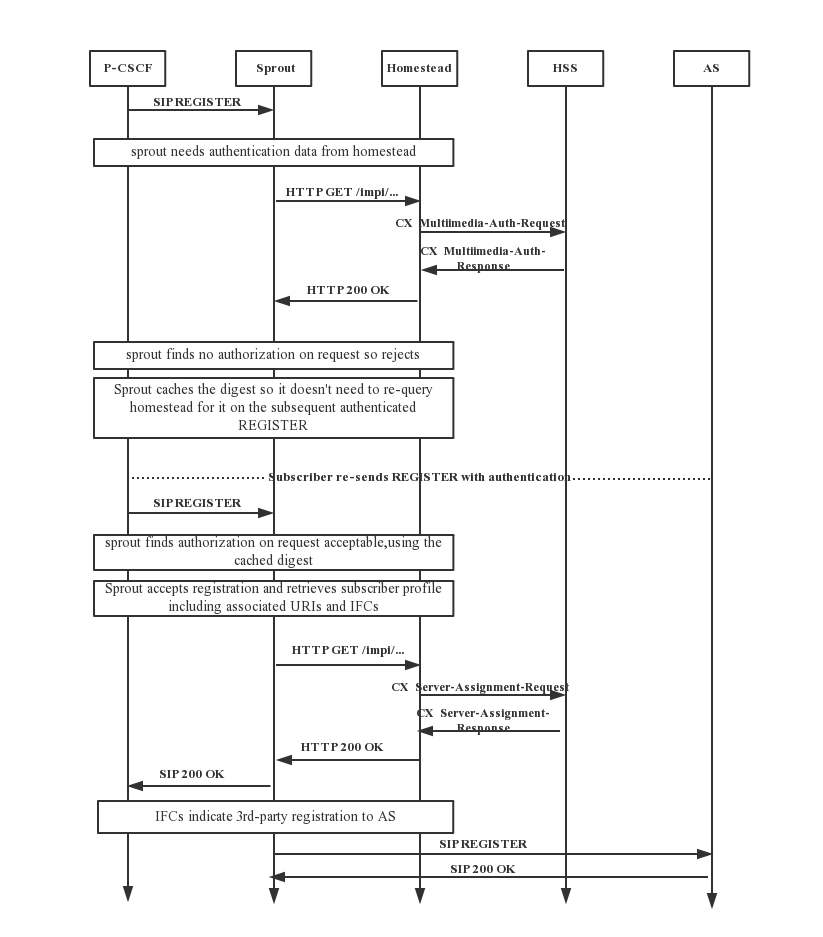
\includegraphics[width=1\textwidth]{clearwater/1.png}
	\bicaption[fig:flow_register]{Clearwater用户注册服务流程图}{Clearwater用户注册服务流程图}{Fig}{Flow of User Registration in Clearwater}
\end{figure}

如图 \ref{fig:flow_register} 所示,当CSCF功能代理 (位于Bono节点中) 向Sprout节点发起注册请求,Sprout 节点需要通过 HTTP 请求向 Homestead 服务(位于Dime节点中)获取用户的认证信息,并根据查询结果来反馈注册结果。此时的服务链的数据流向为 $Bono\longleftrightarrow Sprout\longleftrightarrow Dime$。整个用户注册请求过程中涉及到Bono,Sprout 和Dime这三个功能节点,整个过程可以抽象地看做数据在由这三个节点所构成的服务链中传递。在默认情况下,当Clearwater系统接到注册请求时,系统会从当前运行的这三个功能组的实例中随机地选取来组成服务链来满足服务需求。此时,根据所选取的实例的资源映射情况,我们可以得到不同的实际数据传输路径,整个映射的结果如图\ref{fig:mapping} 所示。图中展示了对于同一条服务链选取了两种不同资源映射组合的情况。这两种映射情况都可以满足注册服务的功能需求,但是由于所选取的虚拟资源不同所以性能上存在差别。由第\ref{related:observe}章中的验证性实验可知,由于所选取的实例间彼此资源的数据传输路径不同,这两种资源映射组合下的服务链的实际性能是不同的。在默认的随机选取的情况下,服务链资源映射的方式是未知的,这给实际服务带来了潜在的性能波动。
\newpage
\begin{figure}[!htp]
	\centering
	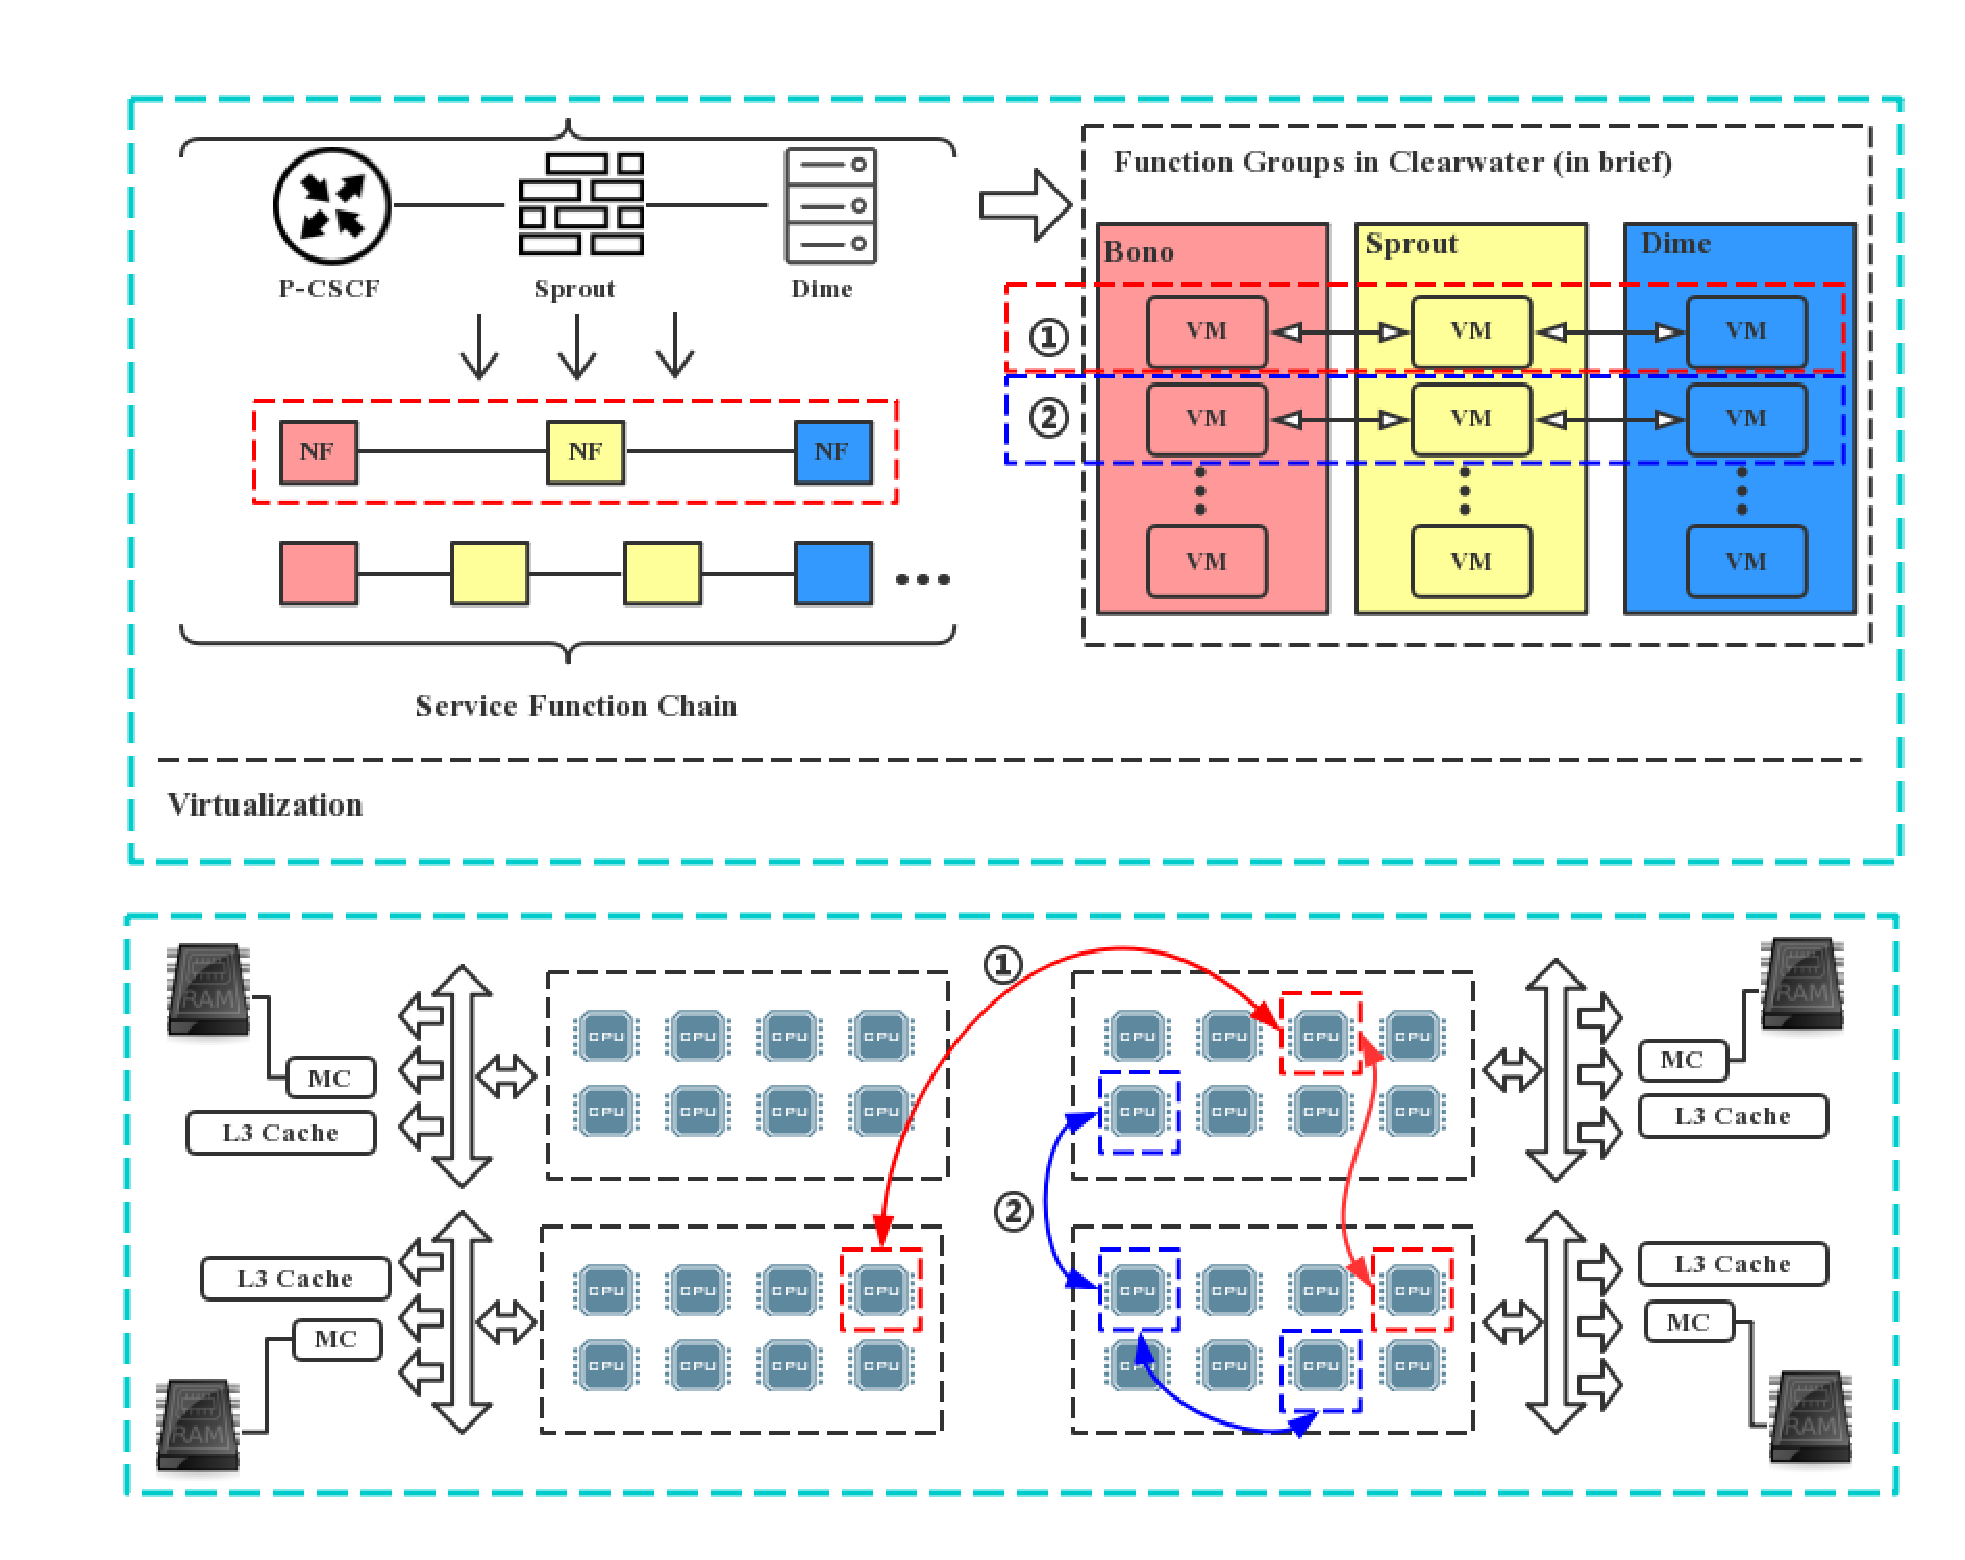
\includegraphics[width=0.8\textwidth]{core.pdf}
	\bicaption[fig:mapping]{Clearwater用户注册服务链资源映射示意图}{Clearwater用户注册服务链资源映射示意图}{Fig}{Resource Mapping Diversity of Clearwater register service}
\end{figure}
从物理机器中实际的数据流角度来看,由于不同的虚拟机实例分配了不同的物理资源,所以数据流的路径会由于所选取实例的不同有所差异。为了更加准确地刻画不同资源组合的服务性能,我们将基于虚拟化的物理资源对IMS服务链进行建模。
\newpage
%本质上这个问题可以被分解为两个步骤:放置网络功能和组织服务链。其中,放置网络功能决定了为了满足当前的服务需求,需要在当前的服务器上部署多少进一步的,为了在实际场景中解决此问题,需要对该问题的前提做一些约束。本文所解决的问题基于以下的假设:

\section{关键概念及模型定义}
为了对虚拟化环境下IMS服务链资源映射问题进行建模,我们需要对一些关键概念进行定义。需要指出的是,在进行服务链资源映射之前,还存在着虚拟机到物理机的映射问题,这一问题已经有大量的研究来解决\citen{chowdhury2009virtual,fischer2013virtual,fajjari2011vne},本文主要针对在运行实例已被初始化完毕前提下的网络功能选取和组链的问题,在后续的实验中本文也在不同的虚拟机到物理机的映射组合下进行了实验,验证本文所提出的优化方法的有效性。为了在实际场景中解决此问题,我们需要对该问题的前提做一些约束。本文所解决的问题基于以下的假设:
\begin{enumerate}
	\item 每个虚拟机实例仅运行一种特定的网络功能应用。网络功能与虚拟机存在多种多样的映射关系,其中,一对一的这种映射关系目前成为了主流。随着轻量级虚拟机的出现\citen{martins2014clickos,manco2017my},一台物理机上所能承载的虚拟机数量得到了极大地提升,因此这种单一虚拟机单一网络功能的模式可以实现复杂的NFV应用。
	\item 每个虚拟机应当专注于处理本身运行的NFV负载,并且尽量避免由于其他无关业务所带来的性能开销。因为我们选择了单核虚拟机并绑定了虚拟CPU到特定的物理CPU从而减少多核调度所带来的额外开销以及上下文切换。
	\item 针对每种特定的网络功能,都有多个运行实例处于待机状态,随时可以根据需求被映射提供服务。
\end{enumerate}
\subsection{相关建模定义}
\textbf{网络功能组}{ }考虑到云计算场景下,各种资源都聚合以资源池的方式对外提供,在IMS场景下尤其是Clearwater平台下也不例外。在这里,我们以集合 $D$ 来表示某种特定网络功能的资源池,也称为网络功能组。

\textbf{服务链}{ }我们用集合 $S$ 代表一条被映射到具体网络上的网络功能服务链。$S$ 由一群有序的虚拟网络功能实例组成 $S = \{f_{a} \to f_{b} \to f_{c}\}$,其中,$f$ 是从特定的网络功能组 $D$ 中(例如 Sprout功能组)选取的某一个运行实例。网络流量根据服务链的连接顺序,依次通过每一个功能节点。

\textbf{多层级映射}{ }如图 \ref{fig:mapping} 所示,除了从服务链描述的抽象逻辑服务链到实际运行的网络功能域中运行实例的映射关系之外,还存在着潜在的从服务链到物理资源的映射。本文用集合 $R^{cpu}$ 表示一台物理机上所有的物理CPU,为了简化问题在上文的叙述中已经假设所有虚拟机仅配置单个虚拟CPU并绑定物理CPU,故在此假设下 $R^{cpu}$ 也可表示所有虚拟CPU的集合。当服务链与运行实例绑定后,服务链与底层物力资源的映射也随之建立。另外,本文使用$R^{mem}$表示一台物理机的所有物理内存。由于虚拟化软件栈的存在,上层的服务链对于所绑定的底层硬件信息并不知晓。但是实际情况是,如同第 \ref{related:observe} 章中验证性实验所示,底层资源之间的选择组合对于整条服务链的性能有着重要影响,所以优化服务链的底层资源组合对提升服务链的整体性能具有重要意义。

因为IMS中主要的负载是数据流量,所以本文使用衡量网络流量的延迟和带宽参数来衡量NFV的网络性能。我们令 $B_{i,j} (i,j \in D, i \neq j)$ 来表示任意两个运行实例(虚拟机)的的网络通信带宽,令 $L_{i,j} (i,j \in D ,i \neq j)$ 来表示两者之间通过真实或者虚拟网络通信的网络通信延迟。按照本文的假设,所有的虚拟机仅配置单个物理核,那么显然也存在一个从 $f \longleftrightarrow m (f \in D, m \in R^{cpu})$的映射。对于服务链上每个虚拟机来说,数据流量将按照串行的顺序沿着数据路径依次通过每个虚拟网络功能节点。

为了衡量整个服务链的带宽和延迟,需要分析任意两个相连的两个实例之间的带宽和延迟。对于带宽而言,根据串行系统的特性,我们选取整个数据链路上最小带宽作为整条链的带宽值如公式 \ref{equ:bandwidth} 所示。 

\begin{equation}
\label{equ:bandwidth}
Bandwidth(S) = \min{(B_{i,i+1} )}, i \in S
\end{equation}

对于任意两个网络功能(虚拟机)之间的通信延迟来说,本文进一步定义了其主要的组成如下:

\begin{equation}
L(i,j) = L_{i,j} + L_{i} + L_{j}, i,j \in D
\end{equation}

其中,$L_{i,j}$ 定义如上文所示表示两个实例的网络传输延迟,$L_{i}$,$L_{j}$ 则分别表示虚拟网络功能处理相关流量而产生的延迟。对于任意一个特定的虚拟网络功能,如果配置了相同的物理资源,则其处理相同网络流量所花费的时间是相同的,也就是说所产生的这部分的延迟是一个与具体服务相关的固定值。

在此基础上我们进一步定义数据流量通过某条服务链 $S$ 在数据路径上的传输延迟为$\Delta Latency(S)$,其定义如下:
\begin{equation}
\Delta Latency(S) = \sum_{i=0,j=i+1}^{\mid S\mid-1}{L_{i,j}}, i\in S
\end{equation}

同理,服务链上累计的数据流量处理延迟为与服务链业务相关的常数$C$。但是$L_{i,j}$这部分的延迟则由于不同物理资源的组合会产生不同的数据传输路径,存在着很大的变化空间。总的来说可以认为,服务链 $S$ 上的传输延迟 $Latency(S)$ 最终定义如公式 \ref{equ:latency} 所示。由公式不难看出,服务链上$S$的传输延迟主要取决于 $L_{i,j}$。

\begin{equation}
\label{equ:latency}
\begin{aligned}
Latency(S) & = \sum_{i=0,j=i+1}^{\mid S\mid-1}{L(i,j)} \\
& = \sum_{i=0,j=i+1}^{\mid S\mid-1}{L_{i,j}}  + C \\
& = \Delta Latency(S) + C, i\in S  		  \\ 
\end{aligned}
\end{equation}

\subsection{网络服务约束定义}
基于上文中已有的模型,这里我们进一步定义模型中的约束,包括服务收益和服务开销。

\textbf{服务收益}{ }一个服务链的服务收益 $P$ 可以被定义为通过一定的映射和调度策略下从所使用的物理资源中收获的定量的服务。参照已经由公式 \ref{equ:latency} 和 \ref{equ:bandwidth} 定义的带宽和延迟,总体的服务收益可以被视为这两个指标的线性和,其中 $\alpha$ 和 $\beta$为线性表达式的系数,由服务的具体需求来调整。例如,对带宽要求要求的服务则$\alpha$的值较大,而对延迟敏感的应用则有较大的 $\beta$ 值。

\begin{equation}                                                             
\label{equ:profit}
P = \alpha*Bandwidth(S) + \beta*(Latency(S)-\Delta Latency(S))
\end{equation}

\textbf{服务开销}{ }我们从所使用的物理资源的角度来定义一条服务链的服务开销。服务链中的运行实体主要是虚拟机,而对于虚拟机而言主要的资源开销为物理CPU,内存,虚拟硬盘和所分配的其他虚拟I/O设备。在本文中,虚拟硬盘和其他虚拟I/O设备与所研究的内容无关故不做考虑,同时服务链所分配的物理资源在理论上不应超过物理机所能提供的物理资源上限。所以,服务开销 $E$ 定义如公式 \ref{equ:expenditure} 所示。

\begin{equation}
\label{equ:expenditure}
\begin{aligned}
E = &\delta * \sum_{i\in S}{r^{cpu}_{i}} + \theta *\sum_{i\in S}{r^{mem}_i}, \\
&\sum_{i\in S}{r^{cpu}_{i}} < R^{cpu},\\
&\sum_{i\in S}{r^{mem}_i} < R^{mem}\\
\end{aligned}
\end{equation}

公式中的$\delta$和$\theta$分别是根据不同应用需求来调节CPU和内存权重的系数。在本文中,结合所使用的实际应用Clearwater服务,我们令 $\delta = 10^{6}$,$\theta = 0.001$ 。同时为了保证服务链物理资源的可用性,本文约束所使用的cpu和内存资源均不超过物理机的资源上限。

从以上定义不难看出,实际的服务开销和服务收益的主要区别在于实际收益中只计算了数据流量在网络功能节点中的处理时间,而实际服务开销则包涵了服务链在传输线路上的传输延迟。


\begin{table}[htb]
	\centering
	\bicaption[tab:variables]{符号表}{符号表}{Table}{Symbols}
	\begin{tabular}{ | l | p{7cm} |}\hline
		\textbf{符号} &							 \textbf{意义}  				\\ 	\hline
		$D$   &	网络功能组  \\ \hline
		$S$	  & 某一网络功能服务链    \\ \hline
	    $R^{cpu}$     & 一台物理机上所有的物理CPU资源   \\ \hline
	    $R^{mem}$     & 一台物理机上所有的内存资源   \\ \hline
	 	$B_{i,j}$	   & 任意两个运行实例(虚拟机)之间的通信带宽   \\ \hline
		$L(i,j)$       & 任意两个运行实例的通信延迟   \\ \hline
		$L_{i}$        &  实例处理数据所产生的延迟  \\ \hline
	    $L_{i,j}$      &  任意两个实例在数据传输路径上所产生的延迟  \\ \hline
	    $C$      &   服务链业务相关的常数\\ \hline
	    $P$      &  一条服务链的服务收益  \\ \hline
	    $E$    &  一条服务链的服务开销  \\ \hline
	    $\alpha$   & 带宽调节参数   \\ \hline
	    $\beta$       & 延迟调节参数   \\ \hline 
	    $\delta$   & CPU资源调节参数   \\ \hline
	    $\theta$      & 内存资源调节参数   \\ \hline   
	\end{tabular}
\end{table}

\newpage
%TODO添加模型有效性的验证
\section{模型参数分析及有效性验证}
\subsection{模型参数分析及获取}
在本章的模型中,我们选取了通信中的延迟和带宽作为衡量服务收益的参数。在实际的虚拟化平台中,每个服务实例都以线程的方式运行在系统中。根据第\ref{intro:IO}章中I/O虚拟化方式的介绍,在以Virtio方式进行网络虚拟化的线程间进行网络通信可以视作两个线程之间进行数据传输。在实际多核非一致性存储访问架构的服务器中,这样的数据传输过程将会受到线程间NUMA资源亲和度影响,已有的研究使用NUMA比率(NUMA ration)\citen{antony2006exploring}或者跳距离(Hop Distance)\citen{tudor2011understanding,pilla2012hierarchical}来描述。但是这样的描述不足以满足本模型中对同时对带宽和延迟的信息需求。为了获取系统运行时准确的资源间数据传输带宽和延迟信息,本文借鉴已有研究的思路\citen{li2013characterization},选择动态采样的方式,通过在运行平台上运行通用的基准测试工具Stream\citen{mccalpin1995stream}和Intel Memory Latency Checker\citen{intelmlc}来测量出所有物理资源间的数据传输的具体通信带宽和传输延迟,将其作为模型的输入参数。数据采样的具体过程见第\ref{imp:sample}章。

使用动态采样的方式来获取带宽和延迟信息有以下两点优势:(1)通过动态采样可以使得本文的模型不依赖硬件平台和操作系统。当硬件平台或者操作系统发生改变时,只需重新运行采样程序,根据测试结果更新输入参数。(2)通过动态采样可以获得更加细粒度的信息。相比于跳距离,采样程序可以获得具体的数据传输带宽大小和传输延迟大小,这样的数据精度使得本文的模型可以更加准确地刻画服务链的物理资源。

\subsection{参数有效性验证}
为了验证动态采样参数的有效性,我们使用一些带宽和延迟敏感的标准负载程序来验证采样结果。通过标准负载应用的程序在不同物理资源下的性能数据与标准动态采样数据相比较,采用非线性回归分析的方法来计算采样参数的拟合程度。假设所选取的资源到所获取的性能之间满足一个非线性的函数关系,我们以采样的部分数据(0号CPU到其他所有CPU节点的访问带宽和延迟)归一化后作为预测值$Y^{\ast}$,以标准负载程序的测试结果归一化作为实测值$Y$,计算其统计学的拟合优度$R^{2}$(无量纲系数,取值范围0到1),以此来判断本文所选取的参数值与真实应用性能的吻合程度。我们利用公式\ref{equ:R2}来计算拟合优度的具体值。根据公式我们可以看出,$R^{2}$的值越接近1则说明拟合程度越高。

\begin{equation}                                                             
\label{equ:R2}
R^{2} = 1 - \sqrt{\frac{\sum_{i= 0}^{N}(Y_{i}-Y_{i}^{\ast})^{2}}{\sum_{i = 0}^{N}Y_{i}^{2}}  }
\end{equation}

本节所使用的标准负载程序和计算结果如表\ref{tab:benchmarks}所示。其中,NPB(NAS Parallel Benchmarks)是一组针对并行计算的性能评估基准测试,由NASA负责开发和维护\citen{bailey1993parallel,wong2003parallel}。而Linkpack测试工具\citen{dongarra2003linpack}是一个通过计算线性方程组来测试系统浮点运算性能的工具。本节中,因为NPB-IS测试会大量使用内存中的数据,属于内存密集型应用,所以我们将带宽参数作为预测值进行了计算。我们选取了IS(Integer Sort)作为具体测试应用,选取的问题规模为Size C。Linpack测试工具则是作为计算密集型应用,用来对比延迟参数,运行时的运算规模设定为了10\%的系统内存。我们使用numactl工具\citen{kleen2005numa}将测试线程与物理资源进行绑定。为了保证实验的有效性,避免出现随机结果,每组实验数据均为多次运行取平均值。

\begin{table}[htb]
	\centering
	\bicaption[tab:benchmarks]{参数有效性验证基准测试工具表}{参数有效性验证基准测试工具表}{Table}{Benchmarks Used for Validation}
	\begin{tabular}{ |c|c|c|c|}\hline
		\textbf{名称} & \textbf{类型}& \textbf{测试参数} & $R^{2}$ \\ 	\hline
		NPB-IS   &	内存密集型 & Size C & 0.90\\ \hline
		Linpack 2.0	  & 计算密集型& Problem Size = 10\% of system memory & 0.86 \\ \hline
	\end{tabular}
\end{table}

通过实验数据统计计算可得带宽参数的拟合优度为0.90,而延迟参数的拟合优度为0.86。基本上可以认为模型中通过动态采样的参数与实际应用所表现出来的性能的变化趋势是一致的,本设计动态采样的参数值可以有效地反映物理资源之间数据传输的性能。

\section{本章小结}
本章主要介绍了针对IMS系统服务链的分析和建模。以Clearwater中的注册服务为例,阐述了服务链的资源映射过程,由此引出了基于IMS服务链的资源映射问题建模,从物理资源间访问的带宽和延迟角度入手,定义了服务链映射的服务开销和服务收益,为接下来的优化算法和优化系统提供模型基础。最后本章对模型中的输入参数进行了有效性验证,利用实际应用的非线性回归的拟合优度来说明所采样参数的有效性。